\documentclass[french]{report}
\usepackage[utf8]{inputenc}
\usepackage[a4paper,total={5.8in, 9in}]{geometry}
\usepackage[T1]{fontenc}
\usepackage{babel}
\usepackage{caption}
\usepackage{hyphenat}
\usepackage{gensymb}
\usepackage{graphicx}
\usepackage{titlesec}
\usepackage{minted}
\usepackage{listings}
\usepackage{enumitem}
\usepackage{xcolor}
\usepackage{amsmath}
\usepackage{amssymb}
\usepackage{hyperref}
\usepackage[cc]{titlepic}
\definecolor{blue}{RGB}{51,131,255}
\definecolor{darkblue}{RGB}{0, 71, 179}
\newcommand\tab[1][1cm]{\hspace*{#1}}
\usepackage[skins]{tcolorbox}
\graphicspath{{img/}}
\hypersetup{
    colorlinks,
    citecolor=black,
    filecolor=black,
    linkcolor=black,
    urlcolor=black
}

\title{{\huge \textbf{Annexe rapport de stage}}\\
{\color{blue} \textbf{Spécifications initiales}}\\
Outil plan de charges\\
{\Large \textit{Application web de gestion}}\\
{\normalsize **Contient des erreurs qui ont été corrigées dans le rapport**}}
\date{\today}
\author{Pierre-Louis Sergent}
\titlepic{
\includegraphics[width=6cm]{logo.png}}
\DeclareMathSizes{12}{30}{16}{12}
\begin{document}
    \maketitle

    \tableofcontents

\chapter{Introduction}
  \section{Objet du document}

Ce document a pour but de présenter les spécifications pour l’application web
de plan de charges. Cette application web viendra améliorer l’outil Excel
proposé par Aurélien Cavalan. Il a pour vocation de permettre une gestion de
l'ensemble des projets de l’activité data de It-link Rennes et ainsi fournir
aux différents responsables une vue d’ensemble sur les projets en cours et sur
la répartition des charges de travail attribuées à chacun des collaborateurs.
Cet outil s’inscrit dans le processus de production.

  \section{Référents}

Ce projet réalisé dans le cadre de mon stage est encadré par le responsable
d’équipe Python/web qui est également mon maître de stage : Alexandre Galodé. Il
en sera le référent technique.\\\\
L’outil Excel sur lequel je vais me baser a été réalisé par Aurélien Cavalan. De
par son statut d'adjoint du responsable d’activité, c’est lui qui est amené le
plus souvent à manipuler l’outil. La rédaction du cahier des charges et la
réalisation du projet s’effectuera donc en collaboration avec ce dernier.

  \section{Phases du projets}

Dans l'ordre chronologique:
\begin{itemize}[label=\textbullet, font=\normalfont \color{blue}]
  \item{Etude de l'outil Excel (étude en autonomie et entretien avec Aurélien Cavalan)}
  \item{Rédaction cahier des charges (URS et SDD)}
  \item{Réalisation, développement}
\end{itemize}

  \section{Terminologie}
\begin{itemize}[label=\textbullet, font=\normalfont \color{blue}]
  \item{PDC : Plan De Charges}
  \item{RdA, RdE, RdP, RT : Responsable d'Activité, d'Equipe, de Projet et Technique}
  \item{TMA : Tierce Maintenance Applicative}
  \item{SDD : Software Design Description (description de la conception logicielle)}
  \item{URS : User Requirements Specification (cahier des charges des exigences utilisateurs)}
\end{itemize}

\chapter{L'outil Excel}
  \section{Présentation générale}

L’outil PDC, comme expliqué dans l’introduction, est un fichier Excel qui permet
d’anticiper les charges à venir, concernant des projets établis ou probables, et
de les répartir entre les différents collaborateurs. Il permet de voir
rapidement les personnes qui travaillent sur tel ou tel projet, à hauteur d’un
certain pourcentage de temps. Il permet également d’avoir une vision globale sur les
charges attribuées à chacun des collaborateurs, afin de ne pas surcharger, ni sous-charger
quelqu’un au moment de la répartition des charges.

\subsection{Feuille Consolidé}

La feuille "Consolidé" affiche par mois, le pourcentage d'occupation attribué à chaque
collaborateur. Le pourcentage est calculé en regardant les feuilles "
Projets", "Probable" et "Autres". Mais aussi en fonction des options
sélectionnées, à savoir : Sans probable, Probable pondéré et Cas majorant. Elle
permet aussi d'afficher une moyenne pour chaque équipe et une moyenne globale.\\
Pour chaque collaborateur le pourcentage par mois est égal à :

\begin{itemize}[label=\textbullet, font=\normalfont \color{blue}]
  \item{=	Projets : Additionne toutes les charges.}
  \item{+	Probable :}
  \begin{itemize}[label=\textbullet]
    \item{Sans probable : comme son nom l’indique on prend seulement en compte
    les projets établis.}
    \item{Probable pondéré : Additionne toutes les charges probables pondérées.
    Charge probable pondérée = charge(en\%) * probabilité}
    \item{Cas majorant : Additionne toutes les charges probables.}
  \end{itemize}
  \item{+ Autres : Additionne toutes les charges pouvant être lié à un congé, une
absence, etc…}
\end{itemize}

\subsection{Feuille Projets}

La feuille "Projets" affiche le plan de charge pour chaque collaborateur en
fonction des projets établis, c’est-à-dire les projets qui ont été commandé.
Chaque projet peut faire l'objet de plusieurs commandes (TMA).\\\\
On peut également voir les charges affectées et les charges RAF en nombre de
jours. Au moment de la commande la quantité de charges est définie. Au tout
début d’une tâche la quantité de charges RAF est donc égale à la quantité commandée.
Puis, à chaque nouveau mois le RdP doit ajuster la case "charges RAF" en fonction de la
quantité de charges réalisée par l’ensemble des collaborateurs (affectés à la
tâche) le mois précédent.\\
La case "charges affectées" est calculée en fonction de la répartition(en \%)
de la tâche entre les collaborateurs.\\\\

\[
CA = \frac{\sum_{i=0,j=0}^n charges_{ij}*\sum_{i=0}^n jours_{i}}{n}
\]

\vspace{0.5cm}

Sachant que :
\begin{itemize}[label=\textbullet, font=\normalfont \color{blue}]
  \item{\emph{CA}, Charges affectées}
  \item{\emph{charges}, pourcentage d'indice i,j dans le tableau.}
  \item{\emph{jours}, nombre de jours ouvrés pour le mois d'indice i dans le tableau.}
  \item{\emph{n}, nombre de mois sur lesquels s'étend la tâche.}
\end {itemize}

\subsection{Feuille Probable}

La feuille "Probable" possède les mêmes caractéristiques que la feuille
"Projets" sauf que chaque  projet possède une probabilité d’être commandé. De
plus, la case "charges RAF" est remplacée par la case "charges estimées".\\ Il
est donc possible de réaliser le plan de charge en  prévision d’un nouveau
projet ou d’une TMA.  Ainsi, si une commande est passée le manager aura déjà
anticipé la répartition des charges.\\\\ Il est important de noter que le client
ne va pas nécessairement commander la même quantité de jours que celle
renseignée dans la case "charges estimées". Dans ce cas, il faudra re-ventiler
les jours entre les collaborateurs dans la feuille Projets. Si la quantité de
jours commandée est la même que celle qui a été estimée, alors on peut recopier
le plan de charges dans la feuille Projets (si le manager est toujours
satisfait de cette répartition).

\subsection{Feuille Autres}

La feuille "Autres" affiche, pour chaque collaborateur le taux d'occupation
associé à des activités qui ne sont pas en lien avec des projets. Par exemple :
absence, alternance, congés, etc…

\subsection{Feuille Commandes}

La feuille "Commandes" affiche toutes les commandes qui ont été prises par les
clients. Cette feuille est importante car elle montre la quantité de charges en
nombre de jours qui a été commandée. Cette quantité est utilisée comme première
donnée dans la feuille "Projets" pour le RAF.

  \section{Utilisation}

\subsection{Quand ?}

Le fichier PDC est utilisé au cours des différentes phases :
\begin{itemize}[label=\textbullet, font=\normalfont \color{blue}]
  \item{\bf{L'avant-vente}}\\
Réalisation du PDC probable dans la feuille "Probable". Première filtre GO/NOGO,
par rapport à la disponibilité des collaborateurs. Puis réalisation du planning
prévisionnel.
  \item{\bf{La commande}}\\
Consolidation du PDC et résolution des éventuels conflits (collaborateur
surchargé,etc).
  \item{\bf{La production}}\\
Suivi du projet, réaffectation de membre au besoin.
\end {itemize}

\vspace{0.5cm}

\subsection{Qui ?}

Le fichier PDC est accessible à tout le monde, mais la plupart du temps c'est le
RdA ou le RdE qui aura à le remplir durant les deux premières phases. Pendant la
phase de production, le RdP pourra également remplir le fichier lui-même en
fonction de l'avancement du projet.

\subsection{Comment ?}

L'avantage du fichier Excel c'est que toutes les cases sont modifiables à tout
moment. Ainsi le PDC possède une forte flexibilité. Cependant l'outil manque
d'automatisme. La création d'un nouveau projet, l'ajout d'un collaborateur, tout
doit se faire à la main. De plus, lors de la réalisation d'un plan de charges,
l'utilisateur doit sans arrêt switcher entre les  différentes feuilles pour
s'assurer que la feuille "Consolidé" est conforme (pas de collaborateur >
100\%).\\\\
A la fin de chaque semaine, une version du fichier est archivée puis stockée dans
le dossier relatif au mois en cours.\\ De plus, mensuellement, le dossier du
mois courant est archivé. Dans la nouvelle version du fichier, on supprime la
première colonne qui correspondait au mois en cours et on ajoute une colonne à
la fin pour toujours avoir une vue tablée sur 13 mensualités.\\\\ L'archivage
sert à garder une trace des PDC pour comparer ce qui a été fait avec ce qui
était prévu auparavant.

  \section{But de l'adaptation en application web}

L'outil Excel possède de nombreux avantages pour assister les différents acteurs
dans le processus de production. Il possède une grande flexibilité et permet de
voir rapidement la répartition entre les collaborateurs et les projets en
cours.\\\\
Cependant une application web permettrait les choses suivantes:
\begin{itemize}[label=\textbullet, font=\normalfont \color{blue}]
  \item{\bf{Automatisation de tâches : }} lors du passage de probable à établi
(récupération du PDC), récupération des charges RAF lorsque l'on rentre une
nouvelle commande, archivage...
  \item{\bf{Application dédiée : }} créer une application consacrée entièrement au
PDC (pour avoir un outil plus "propre").
  \item{\bf{Répartition, pas de limite temporelle : }} dans la version Excel il
est possible de réaliser une répartition seulement pour les 13 mois à venir,
une version web permettrait de s'affranchir de cette limite de temps qui était
imposé par la vue Excel.
  \item{\bf{Facilité d'utilisation :}} utilisation de formulaires, vues
accessibles plus facilement (notamment de la feuille "Consolidé"), pas de
modification "à la main".
\end {itemize}

\chapter{User Requirements Specification}
  \section{Définition}

Les \emph{User Requirements Specification} (URS), ou, le cahier des charges des
exigences de l’utilisateur, a pour but de présenter les exigences utilisateur de
l'application. Il doit contenir une liste exhaustive de ce que l'application sera
en mesure de faire au terme de son développement.

  \section{Priorité}

J'ai décidé de diviser les URS en trois niveaux de priorité afin de bien séparer
les caractéristiques que nous voulons absolument trouver dans l'application finale
et les choses qui pourraient être intéressantes à développer dans le futur.\\
\begin{itemize}[label=\textbullet, font=\normalfont \color{blue}]
  \item{\textbf{FOB : }} fonctionnalité obligatoire\\
  Cette caractéristique doit être incluse dans l'application finale.
  \item{\textbf{FOPT : }} fonctionnalité optionnelle\\
  Cette caractéristique devrait être incluse dans l'application finale sauf si
  contrainte de difficulté ou de temps.
  \item{\textbf{FF : }} fonctionnalité future\\
  Cette caractéristique pourrait être incluse dans l'application finale en
  fonction de l'avancement du projet, ou dans le futur.
\end{itemize}

\vspace{0.5cm}

  \section{Fonctionnalités obligatoires}
\subsection{Explication générale (1)}

Tout comme l’outil Excel, l’application finale devra comporter quatre vues
différentes : \textbf{Projets} (regroupe les feuilles " Projets" et "
Probable"), \textbf{Collaborateurs} (ancienne feuille "Consolidé"),
\textbf{Commandes} et \textbf{Autres}, permettant d’afficher la
répartition (en \%) des charges entre les différents collaborateurs. Chacune de
ces vues aura un système de recherche afin de filtrer en fonction des personnes,
projets ou équipes. Chaque page possèdera des boutons permettant d’ajouter de
nouveaux projets, collaborateurs ou activités (débouchant sur des formulaires),
ainsi que des boutons pour modifier les données déjà présentes. L’intervalle
temporel, pour l’affichage de la vue, devra se faire entre le mois courant et le
même mois de l’année prochaine (soit 13 mois). Une scrollbar horizontale devra
permettre de regarder au-delà de cet intervalle.

\subsection{Organisation (1)}

\begin{itemize}[label=\textbullet, font=\normalfont \color{blue}]
  \item{\textbf{FOB.1 - Affichage vue Projets}}\\
Affichage sous forme de tableau, même colonnes que pour l’outil Excel dans la
feuille "Probable" + nouvelles colonnes "Client" et "Commandé". Contient la
répartition des tâches (en \%), entre les collaborateurs, par mois, ainsi que le
total des charges affectées et des charges RAF. Si le projet est établi alors
le champ "Commandé" vaut 1 sinon il vaut 0.

  \begin{itemize}[label=\textbullet]
    \item{FOB.1.1 - Filtre avec barre de recherche pour les colonnes : }

    \begin{itemize}[label=-]
      \item{Equipe}
      \item{Collaborateur}
      \item{Client}
      \item{Nom projet}
    \end{itemize}

    \item{FOB.1.2 - Boutons principaux : }

    \begin{itemize}[label=-]
      \item{Ajout projet} > \hyperref[sec:1.1]{\emph{formulaire 1.1}}
      \item{Modifier projet} > \hyperref[sec:1.2]{\emph{formulaire 1.2}}
      \item{Supprimer projet} > \hyperref[sec:1.3]{\emph{formulaire 1.3}}
      \item{Ajout collaborateur à un projet (établi ou probable)} > \hyperref[sec:1.4]{\emph{formulaire 1.4}}
    \end{itemize}

    \item{FOB.1.3 - Boutons par ligne : }

    \begin{itemize}[label=-]
      \item{Modifier répartition} > \hyperref[sec:1.5]{\emph{formulaire 1.5}}
      \item{Supprimer collaborateur}
    \end{itemize}

    \item{FOB.1.4 - Affichage liste projets}

  \end{itemize}

  \item{\textbf{FOB.2 - Affichage vue Collaborateurs}}\\
Affichage sous forme de tableau, même colonnes que pour l’outil Excel dans la
feuille "Consolidé". Contient la charge (en \%) de chaque collaborateur par mois
(utilisation des données présentes dans les vues "Projets" et "Autres"). Deuxième
tableau qui affiche la moyenne de répartition pour chaque équipe par mois.

  \begin{itemize}[label=\textbullet]
    \item{FOB.2.1 - Filtre avec barre de recherche pour les colonnes :}

    \begin{itemize}[label=-]
      \item{Equipe}
      \item{Collaborateur}
    \end{itemize}

    \item{FOB.2.2 - Boutons principaux :}

    \begin{itemize}[label=-]
      \item{Ajout collaborateur} > \hyperref[sec:2.1]{\emph{formulaire 2.1}}
    \end{itemize}

    \item{FOB.2.3 - Boutons par ligne :}

    \begin{itemize}[label=-]
      \item{Modifier collaborateur} > \hyperref[sec:2.2]{\emph{formulaire 2.2}}
      \item{Supprimer collaborateur}
    \end{itemize}

  \end{itemize}

  \item{\textbf{FOB.3 - Affichage vue Commandes}}\\
Affichage sous forme de tableau, même colonnes que pour l’outil Excel dans la
feuille "Commandes" + nouvelle colonne "Client". Contient toutes les commandes
passées avec notamment la charge en nombre de jours commandée. Attention, si
une commande est saisie ou supprimée depuis cette page, les vues "Projets" et
"Collaborateurs" seront impactées.

\begin{itemize}[label=\textbullet]
    \item{FOB.3.1 - Filtre avec barre de recherche pour les colonnes :}

    \begin{itemize}[label=-]
      \item{Equipe}
      \item{Client}
      \item{Projet}
    \end{itemize}

    \item{FOB.3.2 - Boutons principaux :}

    \begin{itemize}[label=-]
      \item{Nouvelle commande} > \hyperref[sec:3.1]{\emph{formulaire 3.1}}
    \end{itemize}

    \item{FOB.3.3 - Boutons par ligne :}

    \begin{itemize}[label=-]
      \item{Modifier commande} > \hyperref[sec:3.2]{\emph{formulaire 3.2}}
      \item{Supprimer commande}
    \end{itemize}

  \end{itemize}

  \item{\textbf{FOB.4 - Affichage vue Autres}}\\
Affiche sous forme de tableau, même colonnes que pour l’outil Excel dans la
feuille "Autres". Contient les occupations (en \%) de chaque collaborateur par
mois, qui ne sont pas en lien avec les projets.

\begin{itemize}[label=\textbullet]
  \item{FOB.4.1 - Filtre avec barre de recherche pour les colonnes :}

  \begin{itemize}[label=-]
    \item{Equipe}
    \item{Collaborateur}
    \item{Activité}
  \end{itemize}

  \item{FOB.4.2 - Bouton unique :}

  \begin{itemize}[label=-]
    \item{Ajout activité} > \hyperref[sec:4.1]{\emph{formulaire 4.1}}
  \end{itemize}

  \item{FOB.4.3 - Boutons par ligne :}

  \begin{itemize}[label=-]
    \item{Modifier activité} > \hyperref[sec:4.2]{\emph{formulaire 4.2}}
    \item{Supprimer activité}

  \end{itemize}

\end{itemize}

\end{itemize}

\subsection{Formulaires}

\subsubsection{1.1}
\label{sec:1.1}
\textbf{Nouveau projet} : Ce formulaire sert juste à entrer un projet dans la base de
données, pour le faire entrer dans la vue Projets il faut passer une commande
établie ou probable (\hyperref[sec:3.1]{\emph{formulaire 3.1}})
\\\\ Champs : Client (champ texte), Nom projet (champ texte), RdP (liste
déroulante), RT (liste déroulante)

\subsubsection{1.2}
\label{sec:1.2}
\textbf{Modification d’un projet existant}\\\\ Champs : Nom projet (liste déroulante),
Nouveau nom (champ texte), Nouveau RdP (champ texte), Nouveau RT (champ texte)

\subsubsection{1.3}
\label{sec:1.3}
\textbf{Suppression projet}\\\\
Champs : Nom projet (liste déroulante)

\subsubsection{1.4}
\label{sec:1.4}
\textbf{Ajout collaborateur à un projet établi ou probable}\\\\
Champs : Nom projet (liste déroulante), Référence (liste déroulante), Collaborateur
(liste déroulante)\\\\
Liste répartition (\hyperref[sec:annexe]{voir Annexes}):\\
Bouton unique pour ajouter une nouvelle ligne "template" comme indiquée ci-dessous,\\
Champs : Mois (liste déroulante, forme MM/AA), Pourcentage (liste déroulante)

\subsubsection{1.5}
\label{sec:1.5}
\textbf{Modification répartition}\\\\
Liste répartition (\hyperref[sec:annexe]{voir Annexes}):\\
Bouton unique pour ajouter une nouvelle ligne "template" comme indiquée ci-dessous,\\
Champs : Mois (liste déroulante, forme MM/AA), Pourcentage (liste déroulante)

\subsubsection{2.1}
\label{sec:2.1}
\textbf{Ajout collaborateur}\\\\ Champs : Trigramme (champ texte), Nom (champ texte),
Prénom (champ texte), Rôle (liste déroulante), Equipe (liste déroulante)

\subsubsection{2.2}
\label{sec:2.2}
\textbf{Modifier collaborateur}\\\\ Champs : Nouveau Nom (champ texte), Nouveau Prénom
(champ texte), Nouveau Rôle (liste déroulante), Nouvelle Equipe (liste déroulante)

\subsubsection{3.1}
\label{sec:3.1}
\textbf{Nouvelle commande} : permet de mettre un projet dans la vue "Projets" avec une
répartition initiale\\\\ Champs : Equipe (liste déroulante), Nom projet (liste
déroulante), Date (champ date), Charges (champ nombre entier), Référence (champ texte),
Commentaire (champ texte),\\Etablie ou probable (radio bouton) : si probable,
Nature (champ texte), Probabilité (liste déroulante)\\\\
Liste collaborateur : choix collaborateur (cases à cocher)

\subsubsection{3.2}
\label{sec:3.2}
\textbf{Modification commande}\\\\ Champs : Nouveau nom projet (liste déroulante), Nouvelle
charges (champ nombre entier), Nouvelle référence (champ texte), Nouveau commentaire
(champ texte)\\
Si commande probable : Nouvelle probabilité (liste déroulante), Nouvelle nature (champ texte)

\newpage

\subsubsection{4.1}
\label{sec:4.1}
\textbf{Ajout activité}\\\\
Champs : Collaborateur (liste déroulante), Activité (liste déroulante)\\\\
Liste répartition (\hyperref[sec:annexe]{voir Annexes}):\\
Bouton unique pour ajouter une nouvelle ligne "template" comme indiquée ci-dessous,\\
Champs : Mois (liste déroulante, forme MM/AA), Pourcentage (liste déroulante)


\subsubsection{4.2}
\label{sec:4.2}
\textbf{Modification activité}\\\\
Liste répartition : bouton pour ajouter un nouveau mois,\\
Champs : Mois (liste déroulante, forme MM/AA), Pourcentage (liste déroulante)


  \section{Fonctionnalités optionnelles}
\subsection{Explication générale (2)}

De plus, pour faciliter la lecture, il serait souhaitable d’avoir des options
d’affichage. Notamment dans la vue "Projets", afin d'afficher seulement les
projet établi ou probable. Mais aussi dans la vue "Collaborateurs", ou on
pourrait mettre en place un code couleur, afin de faire ressortir les
collaborateurs qui possède une charge satisfaisante ou bien une charge
supérieure/inférieure à 100\%. Tout comme l’outil Excel, il faudrait également rajouter
des boutons radios pour modifier les charges en fonction de si on prend en
compte les charges probables pondérées ou les charges au cas majorant.\\\\ Pour
faire penser à l’utilisateur de rentrer les charges RAF, on pourrait ajouter une
fenêtre pop-up, au début de chaque mois, pour demander la saisie de la/des nouvelle(s)
valeur(s).\\\\ Concernant les formulaires, afin de faciliter la répartition des
charges (lors de l'ajout d'un collaborateur, ou bien lors de la modification
des pourcentages, formulaires 1.4, 1.5 et 4.1), on voudrait proposer, en
parallèle, une vue dynamique de la page "Collaborateurs", afin que l’utilisateur
voit en direct la répercussion de ses actions. Et aussi, on pourrait proposer
une liste des collaborateurs les plus disponibles pour faciliter la prise de
décision. De plus, on aimerait proposer une récupération automatique du PDC lors
du passage d’un projet probable à un projet établi.

\subsection{Organisation (2)}

\begin{itemize}[label=\textbullet, font=\normalfont \color{blue}]
  \item{\textbf{FOB.1 - Affichage vue Projets}}

  \begin{itemize}[label=\textbullet]
    \item{FOPT.1 - Radio bouton : }

    \begin{itemize}[label=-]
      \item{Filtre avec trois choix : tous ; établis ; probables}
    \end{itemize}

    \item{FOPT.2 - Pop-up :}

    \begin{itemize}[label=-]
      \item{Au début de chaque mois : demande les charges RAF à mettre à jour}
    \end{itemize}

  \end{itemize}

  \item{\textbf{FOB.2 - Affichage vue Collaborateurs : }}

  \begin{itemize}[label=\textbullet]
    \item{FOPT.3 - Radio bouton :}

    \begin{itemize}[label=-]
      \item{Calcul des charges en fonction de trois choix : sans probable ;
       probable pondéré ; cas majorant (100\% de probabilité pour tous les
       projets probables)}
    \end{itemize}

  \end{itemize}

  \item{\textbf{FOPT.4 - Rendre toutes les recherches dynamiques}}

\end{itemize}

\newpage

  \section{Fonctionnalités futures}

\subsection{Explication générale (3)}

Dans le futur, un certain nombre de fonctionnalités seraient utiles. Tout
d’abord un système de login, on demanderait de définir un mot de passe lors du
premier login, de ce fait, seuls le RdA, les RdE et les RdP auraient le droit d’écriture
sur l’application. Les collaborateurs pourraient seulement consulter la
répartition des charges, sans pouvoir ajouter de nouveau projet, ou modifier le PDC, etc… On
pourrait imaginer un système de tickets que les collaborateurs ouvriraient pour
exprimer leurs observations quant à la quantité de travail réel, afin que les RdE/RdP
puissent ajuster les pourcentages et au besoin ajouter un collaborateur sur le
projet.\\\\ Tout comme dans l’outil Excel, on pourrait rajouter des pages
concernant le suivi de projet/production. Sous forme de tableau, avec des
articles résumant l’avancement du projet.\\\\ Pour pouvoir imiter le système
d’archivage de l’outil Excel, il serait utile d’avoir un bouton accessible à
tout moment (dans la barre de navigation) pour exporter le fichier SQL
(utilisation de SQLite) ou bien la database (utilisation de PostgreSQL).\\\\
Enfin, ce n’est pas une fonctionnalité, mais il faudrait que l’application soit
en mesure de gérer les accès concurrentiels pour maintenir la base de données
dans un état cohérent.

\subsection{Organisation (3)}

\begin{itemize}[label=\textbullet, font=\normalfont \color{blue}]
  \item{\textbf{FF.1 - Système de login :}}

  \begin{itemize}[label=\textbullet]
    \item{Demande de mot de passe au premier login}
    \item{Droit d'écriture pour les RdA et RdE/RdP}
  \end{itemize}

  \item{\textbf{FF.2 - Nouvelle vue "Suivi projets" :}}

  \begin{itemize}[label=\textbullet]
    \item{Ajout d'article, mises à jour avancement}
  \end{itemize}

  \item{\textbf{FOB.5 - Affichage barre de navigation onglets : }}

  \begin{itemize}[label=\textbullet]
    \item {FF.3 - Bouton export database}
  \end{itemize}

  \item{\textbf{FF.4 - Gérer les accès concurrentiels}}

\end{itemize}


\chapter{Software Design Description}
  \section{Définition}

  Le \emph{Software Design Description} (SDD), ou la description de la conception
  logicielle, a pour but de présenter l'architecture générale de
  l’application. Ici, la présentation se fera majoritairement à travers deux
  diagrammes : un diagramme de cas d’utilisation et un diagramme de classes. Nous
  finirons cette partie par une réflexion sur l’ergonomie de l’application.\\\\
  L’arborescence ne sera pas détaillée dans cette partie. En effet, l’application
  sera réalisée en utilisant Django, la structure du projet suivra donc les
  standards du framework.

  \section{Diagramme de cas d'utilisation}
  \emph{Cf annexes : figure~\ref{fig:dcu}}\\

  Le diagramme de cas d’utilisation décrit comment les utilisateurs vont pouvoir
interagir avec l’application. Ici, on a supposé que le système de login a été
mis en place, et donc nous avons deux types d’acteurs. D’un côté, l’utilisateur
possédant les droits d’écritures, à savoir, le RdA, les RdE et parfois les RdP.
De l’autre, nous avons les collaborateurs qui pourront seulement consulter les
quatre vues.\\\\ A noter que toutes les flèches pointillées de ce diagramme
représentent des <<include>>, c’est-à-dire que pour réaliser l’action présente
dans une bulle (départ de la flèche pointillée), l’utilisateur doit avoir
réalisé celle présente dans la bulle précédente, vers laquelle pointe la flèche
<<include>>. Les actions que l’utilisateur devra réaliser en premier se trouvent
donc à droite du diagramme.\\\\ Les droits que possèdent les RdA/RdE/RdP
apparaissent clairement, à savoir, le droit d’ajouter de nouveaux projets,
collaborateurs, commandes et activités, puis de les modifier ou supprimer. On
peut également voir que, pour ajouter une commande, il faut que le projet
concerné par cette dernière ait été saisi dans la base de données au préalable
(action "ajout projet").

  \section{Diagramme de classes}
  \emph{Cf annexes : figure~\ref{fig:dc}}\\

   Le diagramme de classes montre les différentes classes qui composent le système
 ainsi que les relations qui existent entre elles. Le modèle proposé ici est
 susceptible d’évoluer au fur et à mesure du développement.\\\\ Il a été décidé
 de distinguer les classes "Projet" et "Commande". Cela met en avant le fait
 que, chaque projet peut faire l’objet de plusieurs commandes distinctes,
 chacune ayant une référence différente. J'ai également décidé de séparer les
 classes "Projet" et "Client" afin d’apporter plus de visibilité au modèle.\\\\
 La classe "RépartitionProjet" prend comme clefs primaires, le trigramme d’un
 collaborateur et un identifiant de commande. Chaque instance de cette classe
 fera donc référence à tous les pourcentages affectés par mois, à un
 collaborateur, concernant une commande précise. Dans l'attribut \emph{liste\_R},
 on trouvera donc une liste de tuples. Dans chaque tuple on trouvera en indice 0 :
 le mois (MM); en indice 1 : l'année (YY); et en indice 2 : le pourcentage. \\\\
 Le principe est le même pour la classe "RépartitionActivité", sauf que l’on
 prend un identifiant d’activité à la place de l’identifiant de commande.

  \section{Ergonomie}

  \emph{Cf annexes : figure~\ref{fig:wf}}\\

  Le design de l’application reprendra les grandes lignes de l’outil Excel.
  C’est-à-dire, les affichages sous forme de tableaux. Les différents boutons
  permettront d’accéder aux différents formulaires, et les barres de recherches
  seront utiles pour filtrer les données. De plus, un \emph{slide button} sera
  présent pour afficher seulement les projets probables (off) ou bien seulement
  les projets établis (on).\\ Pour modifier les répartitions de manière intuitive
  et rapide, des boutons sous formes d’icônes seront placés en face de chaque
  ligne, afin de réaliser les actions directement sur les collaborateurs ciblés.\\


  \emph{Cf annexes : figure~\ref{fig:map}}\\

  Enfin le schéma du mapping indique comment l’utilisateur pourra naviguer sur
  le site. A noter que le schéma a été réalisé en supposant que le système
  de login soit en place. L’utilisateur devra alors se connecter avant de pouvoir
  accéder au reste de l’application.

\chapter{Annexes}
\label{sec:annexe}

\begin{figure}[h]
  \begin{center}
    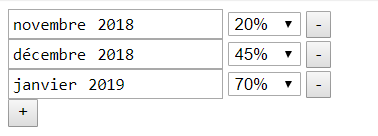
\includegraphics[width=8cm]{ex.png}
    \caption{Liste répartition - formulaires 1.4, 1.5 et 3.1}
    \label{fig:liste_repartition}
  \end{center}
\end{figure}

\begin{figure}[h]
  \begin{center}
    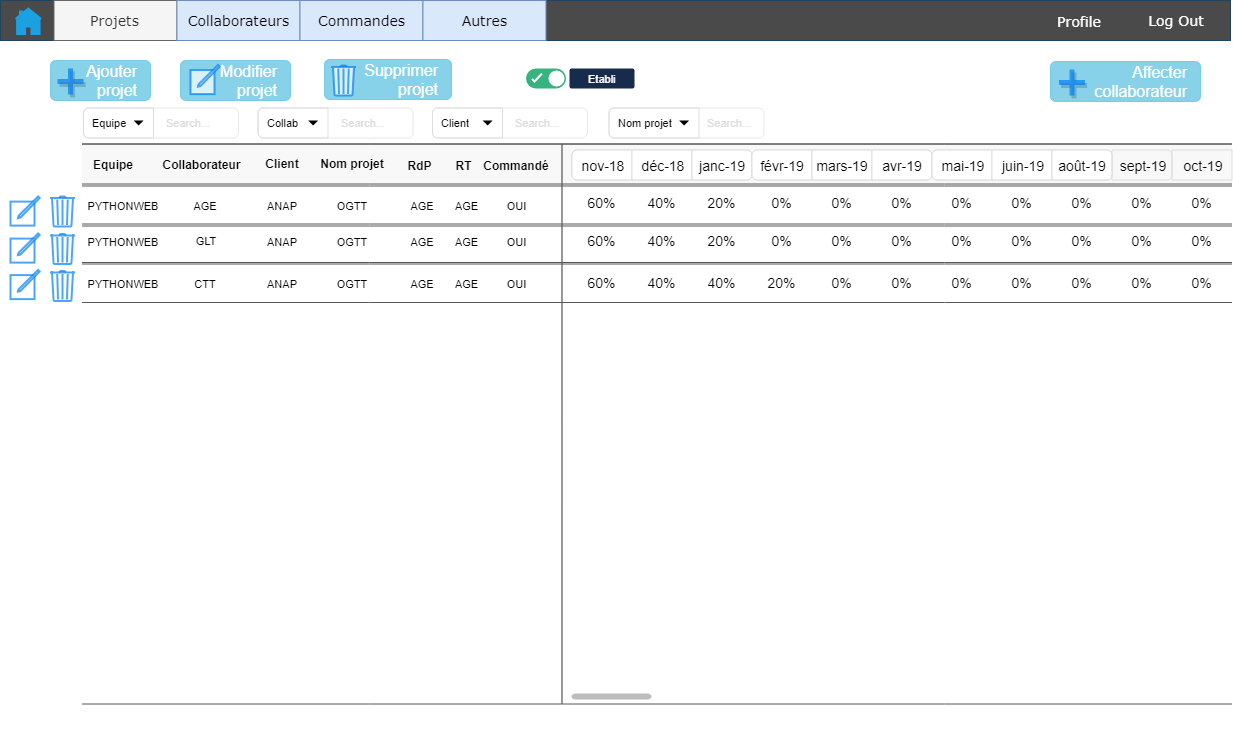
\includegraphics[width=\linewidth]{wireframe.png}
    \caption{Maquette page "Projets"}
    \label{fig:wf}
  \end{center}
\end{figure}

\begin{figure}[h]
  \begin{center}
    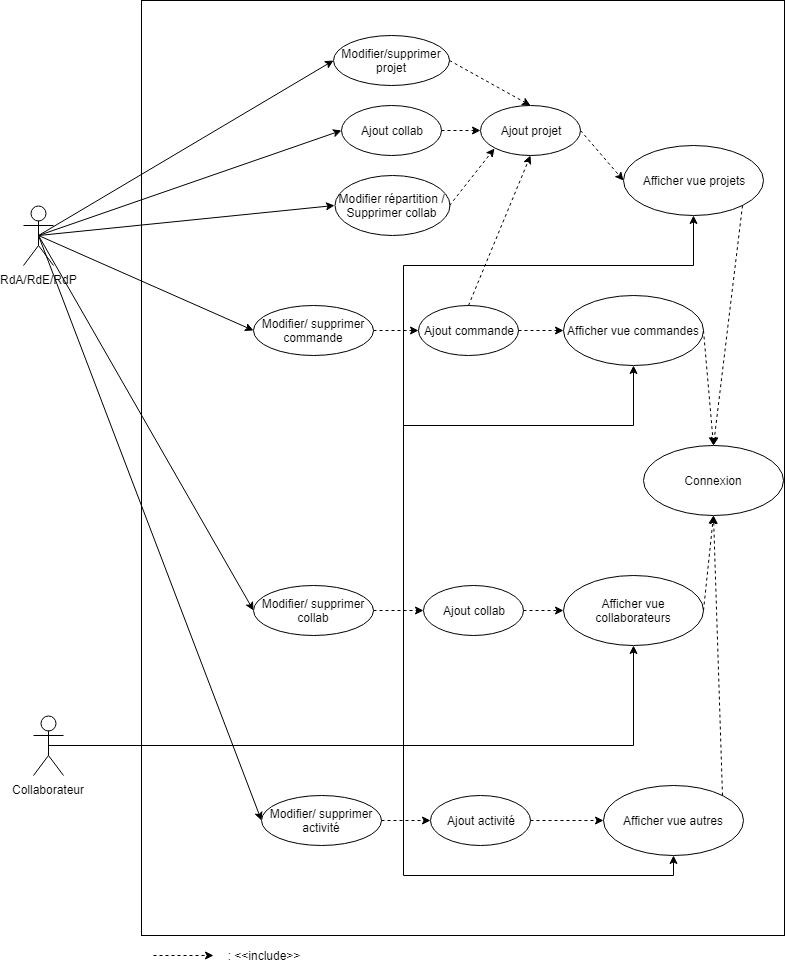
\includegraphics[width=\linewidth]{diagramme_cu.png}
    \caption{Diagramme de cas d'utilisation prenant en compte un login}
    \label{fig:dcu}
  \end{center}
\end{figure}

\begin{figure}[h]
  \begin{center}
    
\includegraphics[width=\linewidth]{diagramme_class.png}
    \caption{Diagramme de classes}
    \label{fig:dc}
  \end{center}
\end{figure}

\begin{figure}[h]
  \begin{center}
    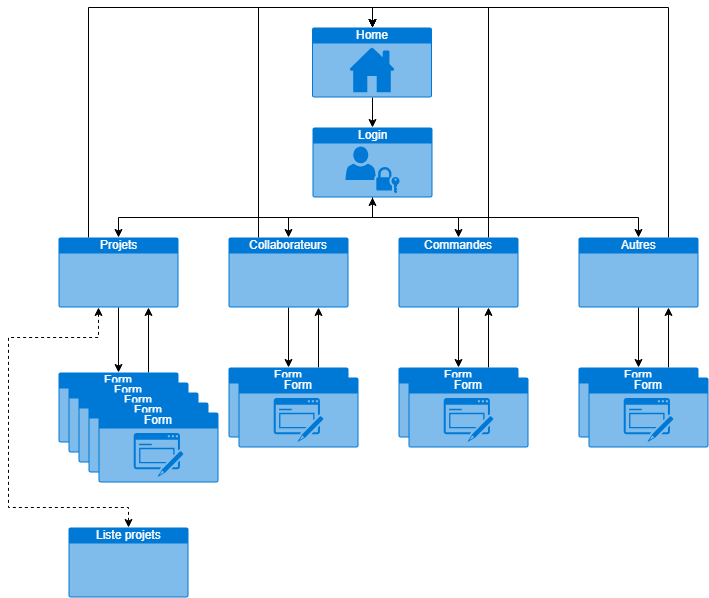
\includegraphics[width=\linewidth]{map.png}
    \caption{Mapping site web}
    \label{fig:map}
  \end{center}
\end{figure}

\end{document}
